\documentclass[letterpaper,serif,tightsqueeze]{module}

\usepackage{parskip}                                                            % Add spacing between paras instead of indents

\title{B3: Palace of the Silver Princess}

% Compress title spacing compared to default

\addtolength{\topmargin}{-0.3cm}
\addtolength{\textheight}{0.7cm}

% Initialise counters

\setcounter{page}{21}
\setcounter{part}{3}
\setcounter{subsection}{44}

\begin{document}

\onecolumn

\begin{center}
Page intentionally left blank.
\end{center}

\twocolumn

locusts are stone gray and may not be noticed until they move or
until the party approaches within 20. They are very nervous and
will flee most of the time rather than fight. They flee by jumping up
to 60. Unfortunately, when they panic their only thought is to
escape. There is a 50\% chance that they will try to flee by jumping
right through the party. If they try to jump through the party,
choose a character at random and roll to see if that character has
been hit. If so, the character takes 1--4 points of damage from being
battered. The locust then flies away.

Cave locusts can also attack and bite for 1--2 points (but not when
they are fleeing). When frightened or attacked, cave locusts make
a loud shrieking noise to warn their fellows. This shriek has a 20\%
chance per round of attracting wandering monsters to investigate.

If cornered, a cave locust will spit a brown gooey substance up to
10' at its attackers. To hit a character, the locust need only make
an attack against armor class 9, no matter what type of armor the
individual is wearing. A character hit by cave locust spittle must
save vs. Poison or be unable to do anything for 1 turn due to the
awful smell. After this time he or she will be used to the smell, but
any character approaching within 5' of the victim must also save or
be violently ill. This effect will last until the spittle is washed off.

The blue glow of the stalactites and stalagmites is caused by a type
of moss. The moss is harmless. It can be used as a weak light
source, casting light up to 10'. If the players search the cave they
will find a small silver statuette of a dragon readying for flight. The
statuette is in a niche along the north wall. The statuette looks the
same as the one found in room 33 (for more details see room 33).

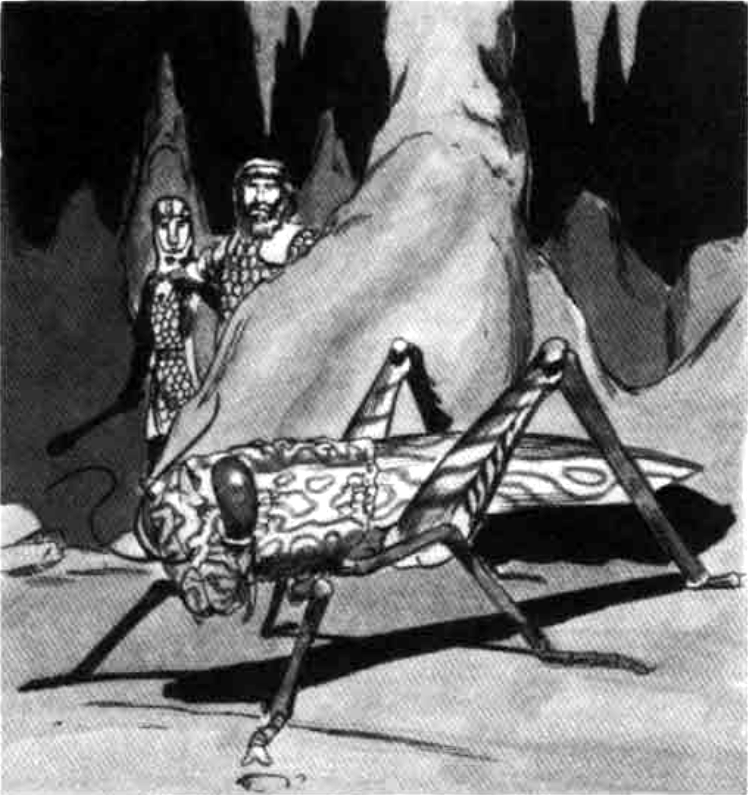
\includegraphics[width=\linewidth]{CaveLocust.png}

\subsection{CAVE POOL}
\begin{boxtext}
A large pool of pitch black water fills the room. You see the glint
of gold coming from the far side of the pool. A hot wind blows
through the cave. Moisture fills the air and tiny beads of water
form on clothing, skin, and hair. The floor is damp and slick.
\end{boxtext}
Once the characters have entered the cave they will be able to see
the crowned head of a large statue of a man. The statue seems to
be made of bronze. The eyes of the statue are small rubies (value
50 gp each). The glint of gold comes from a crown on top of the
statue's head. The crown appears to be made of gold. The statue
really is bronze, but the crown is only gold paint.

The liquid in the pool is a kind of ink. The water of the pool is heated
by hot springs. The hot water absorbs color from a particular kind
of mineral lining the pool. The result is a deep purple ink. Anything
which comes in contact with the ink will be stained purple. Since
the ink is permanent it will have to wear off naturally (1--6 days). It
will not stain non-porous surfaces which do not absorb water very
well (such as steel). The ink will not harm characters.

Once the characters reach the statue they will find that the rubies
can be pried out easily. If the party carefully examines the statue,
there is a 50\% chance they will discover that the head of the statue
can be unscrewed. Hidden inside the head, packed in a protective
oilskin bag, is a \textbf{ring of protection +1}.
\subsection{BLADE TRAP}
At the corner of the corridor is a trap. When a character walks over
a pressure plate in the floor the trap might be sprung. Roll ld6. The
trap will be sprung on a roll of 1. Roll separately for each character
that walks around the corner. If the trap is sprung, a weighted
blade (like a guillotine blade) will fall from the ceiling causing 1--10
points of damage to the person who sprung the trap. The blade is
hidden in the ceiling.
\subsection{TROGLODYTE ROOM}
\begin{boxtext}
In the center of the room you see three human-like reptiles with
short tails, long legs, and a spiny ``comb'' on their heads and
arms. They block the way out.
\end{boxtext}
The human-like reptiles are \stats{troglodyte}{3}{9 each}.
Troglodytes are intelligent. They hate most other creatures and will try to kill
anyone they meet. Hence they will attack on sight. Troglodytes
have a chameleon-like power to blend into their surroundings
(normally they surprise on 1--4 on ld6), but they are not using the
ability at the moment. Troglodytes secrete an oil when fighting
which smells so bad that characters will be nauseated unless they
save vs. Poison. Nauseated characters have a penalty of \minus 2 on their
``to hit'' rolls while in melee combat with the troglodytes.
\subsection{WATCH ROOM}
\begin{boxtext}
This room is higher than the surrounding countryside so that
guards could look out on the surrounding land when standing
watch. There are windows in the west and south walls. You
notice that the red glow still surrounds the palace. In the center
of the room is an iron ladder. The ladder leads to a trap door in
the ceiling. By the south wall you see a statue that looks like a
cleric. He looks frightened and had apparently just finished
scratching a message into the wall. The inscription reads:
\begin{quote}
Evil red eye, malefaction!\\
Sweet music from strings;\\
Priceless Blade of Destruction,\\
Salvation rides on dragon's wings!
\end{quote}
\end{boxtext}
The chief palace cleric had divined the evil intent of Arik when
disaster struck. He hurriedly left the inscription\,---\,clues as to how
to destroy the ruby\,---\,in the faint hope that it might help rescuers.

This trap door is the only way the party can reach the second level
of the dungeon. It is important that the party reach the second level
and finish their mission, but it is also important that they encounter
a number of monsters and traps before reaching the second level.
If they reached the second level too easily the adventure would not
be a challenge. On the other hand, since they must reach the
second level, the DM might consider sending the vision of a Protector
to the party if they cannot find the way to this trap door leading
to the second level.

\onecolumninline{\part{Second Dungeon Level}
\textbf{Wandering Monsters}

The second dungeon level has its own wandering monster table. Check for wandering monsters every other turn. Roll ld6: the party will
encounter a wandering monster if a 1 is rolled. The wandering monster will be first seen 20--120 feet (2d6\x 10') away from the party when
encountered, in any direction and doing anything the DM chooses. To determine exactly which monster is encountered, use the Wandering
Monster Table: Level 2 below:
\begin{center}
\textbf{Wandering Monster Table: Level 2} (Roll ld6)
\end{center}
\begin{wanderingmonsters}
\wanderitem{ghoul}{}
\wanderitem{goblin}{}
\wanderitem{harpy}{1--3}
\wanderitem{hobgoblin}{}
\wanderitem{medusa}{1}
\wanderitem{zombie}{}
\end{wanderingmonsters}

It is suggested that the monsters Harpy and Medusa be encountered no more than once as wandering monsters. If the DM rolls a wandering
monster encounter with a second Harpy or Medusa the DM should choose a wandering monster from the table for Level One instead. This is
because both monsters are very difficult challenges. If encountered too many times, the encounters might upset the play balance.

All the monsters on the second level wandering monster table appear in both editions of the D\&D\registered Basic rules. Only those monsters with
unusual powers are described below.

\textbf{Ghoul}\,---\,A successful attack by a ghoul will paralyze any creature of ogre-size or smaller, except elves, unless the victim saves vs. Paralysis.
Elves are immune to the paralysis, but still take normal damage from a ghoul's attacks. Paralysis lasts for 2--8 turns.

\textbf{Harpy}\,---\,Any character hearing the harpy's song must save vs. Spells or be charmed. Charmed individuals will move toward the harpy,
resisting any attempt to stop them, but not otherwise attacking. If a character successfully saves the character will not be affected by the harpy
song for that encounter. Harpies are resistant to magic and have a +2 on all their saves.

\textbf{Medusa}\,---\,Looking at a medusa will turn a character to stone unless the victim saves vs. Turn to Stone. A medusa can also attack with her
snaky hair. The bite of the snakes is poisonous (save vs. Poison or die in one turn) and when the snakes hit they cause 1-6 points of damage.
Anyone who tries to attack a medusa without looking at it must subtract 4 from their ``to hit'' roll. A medusa is resistant to magic and gains +2 on
saves vs. Spells only, other saving throws are normal.\vspace{-1ex}

\hrulefill
\begin{center}
\textbf{Key to Dungeon Level Two}
\end{center}}
\subsection{WATCH TOWER}
\begin{boxtext}
This watch tower has 6 windows overlooking the surrounding
lands. There is a trap door in the center of the floor. A stone
statue of a guard stands looking out each window. Except for
the statues the room looks empty.
\end{boxtext}
The room is empty except for the statues.
\subsection{PASSAGEWAY}
\begin{boxtext}
As soon as you open the door, bright lights flood the hallway.
You see three swords fighting each other, as if being held by
invisible men.
\end{boxtext}
The fighting swords and bright light is.an illusion pIaced there by
the palace magic-user to frighten intruders who might enter the
palace through the tower. The illusion is triggered by the door
opening without the password ``Argenta'' being spoken. If any
character touches the illusion it will be dispelled.
\subsection{LABORATORY}
\begin{boxtext}
You see a room filled with stuffed animals, shelves filled with
books and scrolls, and jars of powders and herbs. Strange
symbols* are painted on the walls. An iron statue of a warrior
stands in the southeast corner of the room. A polishing cloth is
draped over the warrior's shield.
\end{boxtext}
This room was the palace magic-user's laboratory. The iron statue
is actually a \stats{living_iron_statue}{1}{18}.
Living iron statues have bodies which can absorb iron and steel. When hit, they will take normal
damage, but if a non-magical metal weapon is used, the attacker
must save vs. Spells or the weapon will become stuck in the body of
the living iron statue, and can only be removed if the statue is killed.
\subsection{STOREROOM}
\begin{boxtext}
This small room appears to be empty.
\end{boxtext}
The room once held stores of various sorts but has recently been
cleaned out.
\subsection{MIRABILIS' ROOM}
\begin{boxtext}
A plain bed and a huge wooden desk dominate this sparsely
furnished bedchamber. A broom lies in one corner near a pile of
dirt. A tattered pair of silk bedroom slippers lie on the floor near
the bed. A small nightstand has been overturned. While you
watch, a small black kitten races out from under the bed, bats
one of the slippers around, then runs back under the bed.
\end{boxtext}
\changealignment{panther}{Lawful}
The room is the bedroom of the palace magic-user. The black
kitten is his familiar and pet. Three times a day the kitten can
transform itself into a \stats{panther}{1}{18}.
The transformation lasts 10 rounds. When in kitten form the creature is harmless. Note that
while panthers are usually neutral in alignment, the kitten/panther is lawful because this magical animal is the familiar of a
lawful magic-user.

\end{document}
